\section{Implementacija}
Sastoji se od dva dijela. Prvi dio opisuje igru Texas Hold'em poker te izrada igre u python programskom jeziku. A drugi dio se odnosi na izradu agenta koji treba naučiti igrat ovu igru i biti uspješan na jednoj osnovnoj razini.
\subsection{Implementacija igre}

\subsubsection{Poker}
Jako poznata kartaška igra, nastala u americi, čiji korjeni dosežu do perzijkse igre As-Nas. 
Kroz 19. stoljeće igra se razvijala sa raznim dodacima i varijacijama.
Postaje jako popularna kroz 20. stoljeće kada su se počeli odražvati turniri. Ta popularnost se proširila svijetom uz igranje i održavanje turnira putem interneta, te turniri koji snimaju 
karte svih igrača tako da gledatelji mogu bolje pratit igru. 

Iako postoje razne verzije pokera, svi djele jednaka osnovna pravila igre. Igra se sastoji od 52 igračih karata, koje se mogu promatrati na slici~\ref{fig:poker_cards}, od kojih se 13 karte 4 puta ponavljaju samo sa različitim simbolima. 
Vrijednosti tih 13 karti su: brojevi od 2 do 10, dečko, kraljica, kralj i As. Cilj svakog igrača je sebi složiti najjaču ruku kombinacijom od pet karata.
\\[\intextsep]
\begin{minipage}{\linewidth}
	\centering%
	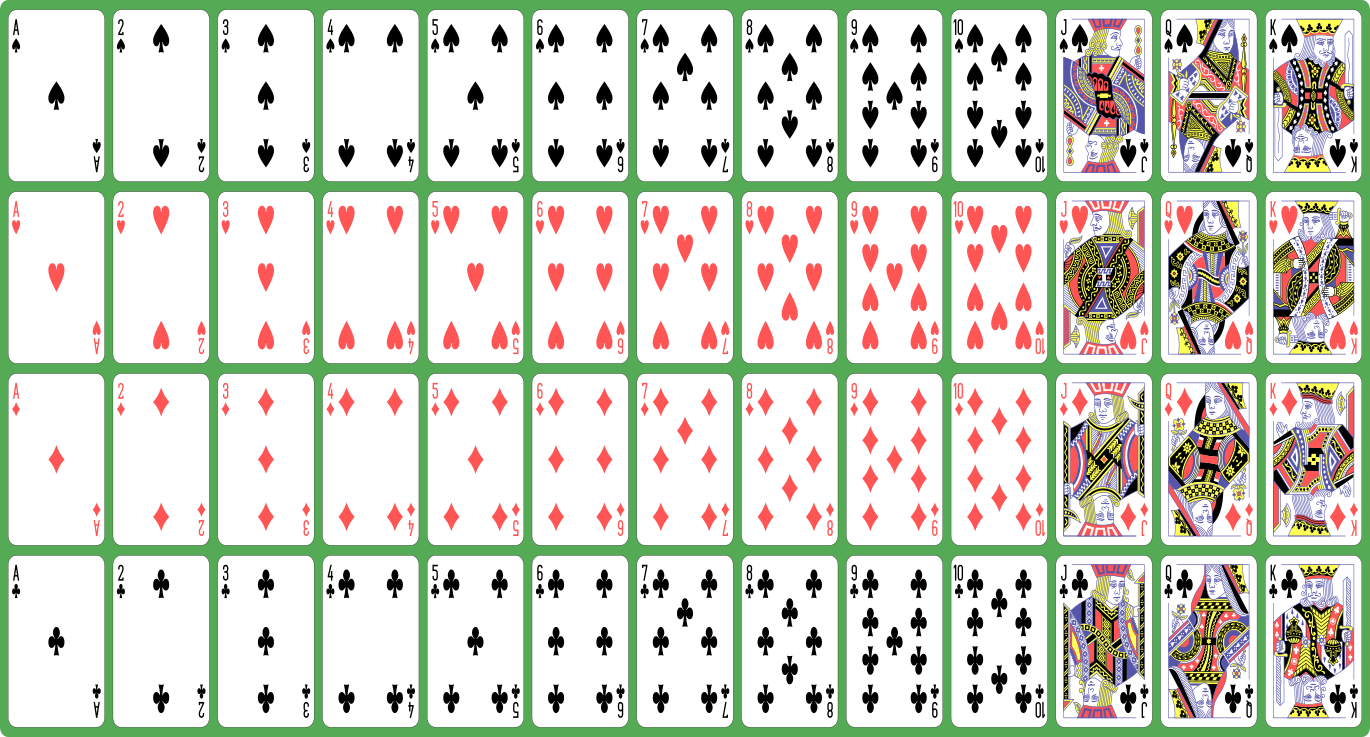
\includegraphics[width=0.8\linewidth,clip=]{images/poker_playing_cards.png}%
	\figcaption{Izgled igračih karata za poker}%
	\label{fig:poker_cards}%
\end{minipage}
\\[\intextsep]

Ruke poredane od najslabije do najjače:
\begin{itemize}
	\item Visoka karta (eng. \textit{high card}): Igrač nije uspijo složiti odgovarajuće kombinacije i gleda se karta sa najjačon vrijednosti. Karte poredane po jačini (od najslabije prema najjače):
	brojevi od 2 do 10 (veći broj znači snažnija karta), dečko, kraljica, kralj pa as.
	
	\item Par (eng. \textit{pair}): Igrač od bilo koje vrijednosti je uspio skupiti dvije iste.
	\item Dva para (eng. \textit{two pairs}): Ruka se sastoji od dvije karte s jednom vrijdnosti i dvije s drugom.
	\item Tris (eng. \textit{tris}): Bilo koja vrijednost 3 puta.
	\item Skala (eng. \textit{straight}): Pet različitih vrijednosti od tako da je svaka sljedeća karta za jednu vrijednost jača od prethodne.
	
	\item Boja (eng. \textit{flush}): Pet karte istog simbola.
	\item Puna kuća (eng. \textit{full house}): Tri karte iste vrijednosti i dvije druge karte istih vrijednosti.
	\item Poker (eng. \textit{poker}): Četiri karte istih vrijednosti.
	\item Skala u boji(eng. \textit{straight flush}): Pet vrijednosti gdje je svaka slijedeća za jednu vrijednost jača od predhodne i svi u istim simbolima.
	
	\item Kraljevska skala u boji (eng. \textit{royal flush}): 10, dečko, kraljica, kralj, as u istim simbolima.
\end{itemize}

\subsubsection{Pravila igre}
Igra koja se implementirala se naziva \emph{Limit Texas hold'em tournament}, i pravila su sljedeća. 
Potrebno je bar dva igrača, tri da bude zanimljivo pa do nekih desetak (nema neke fiksne gornje granice, 
ali najčešće je deset). Prije početka igre svi igrači uplaćuju dogovoreni iznos novca za sudjelovanje u igri, te dobije za uzvrat žetone vrijednosti uloženog novca. Igrači sjedu za ovalnim stolom i jednega od igrača se određuje kao diler. Diler dobije poseban žeton koji ga vidljivo označava kao takvog. Karte se izmišaju i svakom igraču se dodjeli dvije karte, u smjeru kazaljke na satu. Ove dvije karte su za ostale igrače tajna, znači svaki igrač nastoji da jedini vidi te karte, zapamti ih i po mogućnosti do kraja kruga ih drži okrenute naopako na stolu. U prvoj fazi \emph{pre flop} nakon djeljenje karata prvi igrač lijevo od dilera je prisiljen uložit žetone u visini pola vrijednosti minimalnog uloga, taj ulog se naziva \emph{small blind}, a slijedeći ulaže \emph{big blind} cijelokupan minimalni ulog, također prisiljeno. Prisiljeni ulozi služe kako bi u svakom krugu postojala neka dobit, a i da skrati igru koja i onako zna potrajati satima. Ostali igrači nakon njih imaju mogućnost birat hoće pratit (eng. \textit{call}), znači da moraju sve skupa uložit koliki je trenutačni največi ulog, dali će odustat i preklope karte (eng. \textit{fold}), gdje odbacuju karte iz ruku i izključeni su iz igre do kraja kruga ili će povisiti (eng. \textit{raise}) ulog, u kojem slučaju trenutačni ulog postane jednak prošlom plus minimalni iznos za ulaganje. U trenutku kada su ostali igrači napravili potez, prvi igrač do dilera mora nadoplatit ostali isnos za pratit ili izabrat neki od drugih poteza i na kraju igrač koji je mora prisilno uložit minimalni ulog ima mogućnost napravit potez, s tim ako nije bilo povisivanje uloga umisto pratit (eng. \textit{call}) ima potez potvrde (eng. \textit{check}), što znači da nema namjeru povisiti ulog niti izostat iz trenutačnog kruga. Kada svi igrači potvrdu potez diler izbacuje jednu kartu iz igre, reče se da se karta gori (eng. \textit{burn}), te na srid stola okrene 3 karte vidljive svima, to je \emph{flop} faza. 
Karte okrenute na srid stola su karte zajednice (eng. \textit{community cards}) i svaki igrač ima pravo svoju ruku od pet karata složit sa bilo kakvom kombinacijom svoje vlastite ruke i kartama zajednice. Slijedi potez svakog igrača, međutim u ostalim fazama nema prislinog ulaganja. U \emph{turn} fazi diler opet izbacuje kartu i okrene sljedeću na stol, ponovno svi igrači određuju svoji potezi. \emph{River} faza je identična \emph{turn} fazi, tako da na kraju su pet karte okrenuti na sredini stola i bar dva igrača u igri. Sada igrači okreću karte i izjasnu koju kombinaciju su sebi složili, i igrač sa najjačon kombinacijon kupi ukupan ulog (eng. \textit{pot}), ili ako imaju nekoliko igrači istu jačinu onda ga djele. Ako se u bilo kojoj fazi dogodi da svi osim jednog igrača odustaju, preskaču se ostale faze i igrač skuplja ukupni ulog. Postoji još poseban potez ulaganja sve (eng. \textit{all in}) gdje igrač kada nema dovoljno žetonih za uložit, ulaže sve što ima i u slučaju gubitka izbačen je iz igre. Dobitnik je igrač koji zadnji ostaje u igri i nagrada mu ukupan uplaćeni ulog svih igrača. Pošto je igra nepotpuno informirana igra postoji mogućnost blefiranja gdje igrač sa lošom rukom ulaže i/ili diže ulog da stvori dojam da ima jaku ruku na račun kojeg će neki ili svi ostali igrači odustati u trenutačnom krugu.


\emph{Limit} označava da je svaki ulog fiksan i u svakoj fazi su dozvoljena tri ponovno povisivanje uloga (eng. \textit{reraise}), gdje za razliku od \emph{no limit} igrač može povisiti najmanje minimalan ulog a najviše koliko hoće te nema ograničen broj ponovnog povisivanje uloga.

\emph{Texas hold'em} je ovaj način igre sa dvije tajnim kartama i pet javnih, gdje u klasičnom pokeru svaki igrač dobije pet karte (koje su drugim igračima tajna) im pravo izbacit nijednu, nekoliko ili sve karte i onoliko koliko je izbaci dobije novih, te postaje konačna ruka.

\emph{Tournament} podrazumjeva da svi igrači na početku uplate jednak iznos i igra se dok svi ispadnu osim jednog, dok u \emph{cash game} može igrač ponovno kupit žetone za nastavit igrat, može odustat od igre 
iako nije izgubi sve žetone te ih unovčit mogu i čak naknadno doć novi igrači.

\subsubsection{Program}
Pisane su klase koje predstavljaju karte i špil. Klasa \pythoninline{Card}, koja je dana u ispisu~\ref{poker_card}, predstavlja jednu kartu koja ima 3 vrijednosti: oznaku, symbol i vrijednost. Dok klasa \pythoninline{Deck}, koja je dana u ispisu~\ref{poker_deck} stvara špil od 52 odgovarajućih karti za poker te implementira metode za mješanje dijeljenje i izbacivanje kartih.

\pythonexternal[caption={Klasa karta}, label=poker_card]{code/poker_card.py}
\pythonexternal[caption={Klasa špil}, label=poker_deck]{code/poker_deck.py}

Svi igrači koji žele sudjelovat u poker turniru moraju biti nasljeđeni od abstraktne bazne klase \pythoninline{Player} koja je prikazana u ispisu~\ref{poker_base_player}. 

\pythonexternal[caption={Bazna klasa igrač}, label=poker_base_player]{code/player.py}

Bazna klasa prima količinu žetonih kao parametar u konstruktor, implementira osnovne operacije svakog igrača, koje su: primanje žetonih, trošenje žetonih, primanje karte, pokazivanje ruke, uništavanje ruke i prikaz vrijednosti žetonih. Bazna klasa definira abstraktnu metodu \pythoninline{make_move} za odrađivanje akcije koja prima trenutačno stanje igre te niz mogućih, odnosno, dozvoljenih akcija. Trebala bi vratit jedan od akcija koja se nalazi u nizu dozvoljenih. U suštini bi trebao inteligentni agent na osnovu određenog stanja u igri donijet odluku o najboljem sljedećem potezu. Ostavlja se fleksibilnost za buduće pokuse gdje se na osnovu broj informacija o okruženju, odnosno, stanja u igri, mjeri kvalitetu odluke agenta o sljedećem koraku (agent se smatra inteligentijim kad sa što manje informacija donese dobru odluku). 


Klasa \pythoninline{Table} u konstruktor prima niz klasa \pythoninline{Player} i u konstruktoru inicijalizira objekt za svakog igrača. Koristi vlastitu implementaciju igrača, koja je kao pomoćna klasa za radom sa igračima za stolom. 

%\pythonexternal[caption={Pomoćna klasa igrači za stolom}, label=poker_table_players]{code/table_players.py}

Glavni dio cijele igre je klasa \pythoninline{Table}, brine se o raspored igre te primjenjuje pravila limit texas hold 'em turniru. Prima niz klasa kao ulazni parametar u konstruktor. Provjerava dali su sve klase nasljeđene od bazne klase igrača, inicijalizira sve igrače sa prosljeđenim klasama, dodjeljiva im žetone i pokreće igru. Stol posjeduje vlastitu klasu igrača koja enkapsulira baznu klasu, te dodatne podatke koje služe za praćenje same igre. Ova pomoćna klasa prikazana je ispisom~\ref{poker_table_players} u dodatku. Implementirana stilom klasične povezane liste, s kojom se omogućuje zatvaranje kruga, odnostno igrač nakon posljednog je prvi. Dodatno na ovaj način nije potrebno pratiti tko je trenutačno diler, jer je to uvijek glava liste. Za intuitivno korištenje ove klase u petljama potrebno je implementirati pythonove metode \pythoninline{__iter__} i \pythoninline{__next__} koje se brinu i o tome da petlja završava sa posljednjim igračom. Podatke koje klasa čuva za svakog igrača su: referenca na objekt igrača, ime klase od tog objekta, ime igrača, trenutačni ulog, sveokupni ulog, bodove (odnosu se na kraju svakog kruga ovisno o jačini ruke dobije određeni broj bodova), dali je aktivan (u smislu trenutačnog kruga, dali aktivno sudjeluje u ulagnje/povisivanje uloga itd.), posljedni donešeni potez, krajna ruka i kojeg je tipa ta ruka. Ova klasa implementira povezanu listu tako da ima referencu na sljedećeg igrača (što olakšava držanje redosljeda igrača te mjenjanje dilera). Nakon što stol rasporedi igrače, započinje sa turnirom, prolazi kroz sve faze igre dok ne ostane samo jedan igrač. Prati ulaganja svih igrača, i na kraju dijeli ukupni ulog odgovarajućim igračima. Klasa za igrače za stolom smještena je u datotečnom sustavu unutar direktorija za stol. Namjena je usko vezana za igru tako da njen domet nebi smijo prelaziti samog stola. Kvalitetan software bi se trebao sastojati od neovisnih elementih, što omogućuje jednostavnije testiranje svakog elementa te razmjena ili dodavanje novih elementih. Iako se dosta toga u ovoj klasi razdvojilo (kao npr. izrađena je odvojena klasa koja određuje jačinu krajne ruke), i dalje ima prostora za refaktoriranje. Tu bi sljedeći korak bio izbaciti podjelu žetona na kraju svakog kruga u zasebnu klasu i tako rasteretit klasu stola. Najkompleksnija funkcija cijele igre je na kraju svakog kruga koja dijeli žetone dobitnicima. Pošto mora pokriti sve mogućnosti, dosta problematično postaje kada je nekom ili nekoliko igračima posljedni potez \emph{all in}, tada nastaju nekoliko razina dobitnika te se svakom dobitniku mora izračunat točan dobitak. Postoje slučajeve gdje nakon djeljenje \emph{pota} ostaju žetonu jer ih nije moguće podjelit na broj dobitnika. U tom slučaju svaka kuća ima svoja pravila i većinom se igra po nekom dogovoru za taj slučaj. Ode se taj ostatak prenese u sljedeći krug, igra se normalno i na kraju dobitnik tog kruga, ili dobitnici ako je moguće među njima podilit bez ostatka, pokupi ostatak od predhodnog kruga. Kroz izradu igre, je klasa \pythoninline{Table} poprimila preveliku odgovornost i previše stvari se odvijaju u toj klasi, da se kroz refaktoriranje izdvojilo klasu koja računa jačinu ruke. Bodovni sustav je osmišljen tako da najjača ruka nekog tipa ruke ima manje bodova od najslabije ruke jačeg tipa. U dodatku se nalazi klasa koja pronalazi konačnu ruku i dana je u ispisu~\ref{poker_strongest_final_hand_finder}. Ova se klasa uglavnon sastoji od statičkih metoda, nema potrebe da išta drži za sebe. Prima proizvoljan niz karte i vraća kombinaciju kartih koja predstavlja najjaču ruku. Uspoređuje ruku sa najjačon prema najslabijon, tako da u trenutku kada se pronađe odgovarajuća ruka nije više potrebno dalje povjeravat nego se je vrati. Nije potrebno inicijalizirat objekt ove klase nego se funkcije direktno pozivaju priko klase. Koeficijent svake vrste ruke dan je ispisom~\ref{poker_final_hand_type}.

\pythonexternal[caption={Koeficijenti vrste ruke}, label=poker_final_hand_type]{code/final_hand_type.py}

Vrijedi još spomenuti prikaz informacije o igri, gdje se implementirao uzorak dizajna promatrača (eng. \textit{observer design pattern}) isto poznat kao objava i preplata (eng. \textit{publish and subscribe}). Koristi se najčešće kada postoji potreba na više elemente zahtijevaju iste informacije te promjene tih informacije, kao npr. za prikaz na drugačiji način. Efektivno razdvaja logiku izvršavanja i prikaz informacija. Sastoji se od dvije komponente, od objavitelj koji drži sve preplatitelje i samog preplatitelja. Objavitelj omogućuje dodavanje i odstranivanje preplatitelje te obavještavanje preplatitelje o promjene. Svaki preplatitelj sam za sebe definira na koji način će koristiti informacije i kako se promjene izražavaju. Implementacija objavitelja u python k\^odu prikazan je ispisom~\ref{poker_publisher}. Stime se oslobodila klasa \pythoninline{Table} da se brine o bilo kakvim načinom za prikaz informacije o stanju igre, samo mora definirati metode koje dodaju i odstranivaju preplatitelje i u određene trenutke pozvati \pythoninline{notify} funkciju od objavitelja.

\pythonexternal[caption={Objavitelj}, label=poker_publisher]{code/publisher.py}

Implementirala su se dva preplatitelja, jedan koji ispisuje stanje u terminal a drugi koji zapisuje stanje u tekstualnu datoteku. U buduće bi se moglo dodati neki grafički prikaz stanja što ovaj uzorak dizajna omogućuje bez da se mijenja postojeći k\^od, samo se dodaje nova klasa koja nasljeđuje \pythoninline{BaseSubscriber}.

Za osiguranje sigurnosti k\^oda pisani su testovi, te u slučaju izmjene ili dodatka novih funkcionalnosti, prikazuju dali su izmjene utjecali negativno na postojeći k\^od. Postoji disciplina razvoj upravljan testovima (eng. \textit{test driven development}), u kojemu nije dozvoljno pisati iti jednu liniju produkcijskog k\^oda prije nego je napisan test koji ne prolazi i ne piše se niti jedna linija testnog k\^oda dok postoji test koji ne prolazi. Nakon što postoji test koji neprolazi piše se produkcijski k\^od koji omogućuje prolaznost testa i vraća se pisanje novog testa. Nažalost ova disciplina nije primjenjena u ovom projektu, iz razloga, što je potrebno, kako u bilo kojoj disciplini, bar nekoliko mjeseci iskustva kako bi se efektivno primjenila. Bez obzira nije se izostavilo važnost testova, pa su se za najvažnije funkcije implementirale testove, iz jednog razloga za provjeru dali kod radi uredu i iz drugog, da se za sve buduće promjene može provjeriti ispravnost. Testovi su poslužili u nekoliko trenutaka a pogotovo u fazi refaktoriranje k\^oda. Za testiranje jedinica (eng: \textit{unit test}) koristilo se pythonov modul unittest iz razloga jer se nalazi u pythonovoj standardnoj biblioteci, nije potrebna ikakva instalacija i može se direktno koristit. Kreiran je direktorij test, te po konvenciji se osigurava da se ime svake skripte testa započinje sa \pythoninline{test_}. Svaka klasa koja testira neku jedinicu mora bit nasljeđena od \pythoninline{unittest.TestCase}, i ime svake funkcije koja testira jedinicu također započinje sa \pythoninline{test_}. \pythoninline{TestCase} klasa ima implementirane funkcije za provjeru kao što su assertEqual, assertTrue, assertFalse, ..., također implementiranu funkciju \pythoninline{setUp} koja se izvršava prije svake testne funkcije. U toj funkciji se pripremaju objekt/i za testiranje keko se nebi trebalo u svakoj funkciji ponavljat iste postupke. Iako se testne funkcije nalaze u istoj klasi objekti kreirani u \pythoninline{setUp} funkciji se ne djeli među testnim funkcijama nego se za svaku funkciju kreira novi. Funkcija \pythoninline{setUp} se eksplicitno ne poziva nego sve to obavlja bazna klasa \pythoninline{TestCase} u pozadini. U dodatku se može promatrati potpuni primjer jednog testa koji je dan u ispisu~\ref{python_test_case}. Osnovna pravila koje bi se trebali svi testovi držati su, kao prvo moraju biti brzi. Brzo u izvršavanju i prikazivanje rezultata. Testovi kojima treba puno vrimena se ne izvršavaju često i kao posljedica pojavljivaju se greške u k\^odu. Moraju biti neovisni jedni od drugima, znači ne smije niti jedan test postojat koji se nemože pokrenuti prije nego se pokrene neki drugi test. U bilo kojemu trenutku bi trebala postojat mogućnost pokrenut bilo koji test u bilo kojem redosljedu. Trebali bi se moći pokrenuti u bilo kakvom okruženju. Dodatno svi testovi moraju samostalno prikazat dali je test prošao ili ne i koji nije prošao. Test ne smije ikakvu informaciju izbaciti gdje je potrebna ljudska evaluacija rezultata.

\subsubsection{Protivnici}
Za dokazivanje da inteligentni agent napreduje i zna igrati igru, potrebno je modelirati nekog protivnika na osnovu čega se mogu donjeti ove zaključke. Najosnovniji protivnik sa čime se miri agent u bilo kojem području strojnog učenja jest agent koji donosi nasumične odluke. U slučaju pokera agent prima dozvoljene akcije u nekom stanju te nasumično izabere jednu od njih. Specifično za poker je ovo pre loš protivnik, jer je u bilo kojemu stanju među dozvoljenim akcijama se nalazi \textit{fold}. Jako su rijetke situacije kada igrač odustane od trenutačnog kruga a da nije niko povisija ulog. Dodatno potpuno nasumičnim biranjem akcija se češće prekida krug, jer su svi igrači osim jednoga odustali, što znači da agent rijetko posjećuje posljedno stanje kruga u kojemu se ocjenuju ruke. Iz ovog razloga je osnovni protivnik, protiv kojega se inteligentni agent mora iskazati, polu nasumični. Polu nasumični protivnik će slučajnim odabirom izabrati akciju \textit{fold} samo u slučaju kada se povisio ulog. Dodatno se implementirao algoritam sa nekom heuristikom. Početnu ruku u \textit{preflop} fazi kada još nema karte na stolu se boduje na osnovu tablice koju su složili David Skalinsky and Mason Malmuth~\cite{starting_hand_groups}. Tablica grupira sve početne ruke u razine od najjače prema najslabije. U ostalim fazam se računa jačina ruke metodama koje se naslanjaju na rad: Opponent modeling in poker~\cite{EHS}. U radu se opisuje izračun učinkovite jačine ruke (eng. \textit{effective hand strength}) koja je dana formulom~\ref{eq:ehs}.

\begin{equation}\label{eq:ehs}
EHS = HS \cdot (1 - NPOT) + (1 - HS) \cdot PPOT
\end{equation}

Gdje je $HS$ trenutačna jačina ruke, neuzimajući u obzir poboljšanje ili pogoršanje buduće ruke. $NPOT$ je negativni potencijal koji uzima u obzir pogoršanje buduće ruke a $PPOT$ pozitivni potencijal koji zadrži poboljšanje buduće ruke. Potpuna implementacija ove formule je računalna jako zahtjevna. Za izračun trenutačne jačine ruke potrebno je generirati sve moguće protivničkove karte u ruci te usporediti jačinu sa svojom rukom, što je još prihvatljivo. Međutim za izračun pozitivnog i negativnog potencijala potrebno je generirati za svaku sljedeću fazu sve moguće karte koje se mogu okrenuti na stolu i usporediti sve moguće protivničkove ruke sa svojom. Pa se iz tog razloga odlučilo koristit samo trenutačnu jačinu ruke.

\subsection{Implementacija agenta}
Agent se implementirao pomoću PyTorch radnog okvira. Definirani hiperparametri su globalno za cijelu klasu, za brzo i jednostavno mijenjanje. U konstruktoru se provjerava dali postoji cuda sposobna grafička procesorska jedinica i pohranjuje tu informaciju na sljedeći način \pythoninline{self._device = 'cuda' if torch.cuda.is_available() else 'cpu'}. Stvaranje same umjetne neuronske mreže dana je ispisom~\ref{simple_dqn_create_network}, gdje se može primjetiti kako na osnovi varijable \pythoninline{self._device} sadržaj neuronske mreže pohranjuje u odgovarajućoj radnoj memoriji. Kako grafička procesorska jedinica ima svoju vlastitu radnu memoriju potrebno je u njoj inicijalizirati neuronsku mrežu u slučaju da se je želi koristiti za treniranje.

\pythonexternal[caption={Stvaranje neuronske mreže za DQN}, label=simple_dqn_create_network]{code/simple_dqn_create_network.py}

Neuronska mreža je jako jednostavna, ima samo dva skrivena potpuno povezana sloja sa ispravljenom linearnom jedinicom (eng. \textit{rectified linear unit}) kao aktivaciju. Ova aktivacija za svaki element koji je negativan postavlja na nulu, a pozitivne ne dira. Sastavljena neuronska mreža se pohranjuje u variablu \pythoninline{self._policy_net}. Kroz trening se neuronska mreža ažurira na kraju svakog kruga, što znači da se svi potezi do tada moraju na neki način pamtiti. Ovaj način se pokaza da ubrzaje treniranje. Osim poteza se pamti cijelokupno iskustvo u određenemu stanju koje se sastoji od predhodno stanje, prethodna akcija, prethodne moguće akcije i sljedeće stanje. Funkcija koja ažurira neuronsku mrežu prikazana je u ispisu~\ref{simple_dqn_update_network}.

\pythonexternal[caption={Ažuriranje neuronske mreže za DQN}, label=simple_dqn_update_network]{code/simple_dqn_update_network.py}

Nagrada koja se prosljeđuje je razlika žetonih prije početka kruga i nakon, tako da ako je razlika pozitivna znači da je agent pobjiedio, a ako je negativna onda je izgubio. Funkcija iz PyTorch biblioteke koja priprema neuronsku mrežu za treniranje se poziva sa \pythoninline{self._policy_net.train()}. Nakon toga se dohvaćaju i pripremaju iskustva. Funkcija \pythoninline{torch.cat} spaja sve elemente u nizu u jedan tensor, jer je to što se očekuje kao ulaz pozivanje neuronske mreže. U ovom koraku se dohvaćaju sve q-vrijednosti za predhodno stanje tako da se poziva neuronska mreža sa predhodnim stanjem, što se u slučaju običnog q-učenja sa tablicom jednostavno radilo indeksiranjem u odrećeni redak. Sljedeća funkcija \pythoninline{_generate_target_preds} stvara novo izračunate q-vrijednosti za akcije koje se ažuriraju, a to su akcije koje su izabrane u tom stanju. Ostale akcije se ne mijenjaju, što je usporedivo kod običnog q-učenja gdje se ažurira samo jedna ćelija u tablici. Stvaranje ažurirane q-vrijednosti dan je u ispisu~\ref{simple_dqn_generate_target_preds}. Gubitak se računa pomoću funkcije srednje kvadratne pogreške, koja pruža PyTorch \pythoninline{torch.nn.MSELoss()}, na osnovu čega se u povratnoj propagaciji ažuriraju parametri u mreži. PyTorchev \pythoninline{torch.optim} sadrži klase koje su zadužene za ažuriranje neuronske mreže, a u ovom slučaju se koristio \pythoninline{torch.optim.Adam}. Sama inicijalizacija optimizatora ze izvršila u konstruktoru klase naredbom \pythoninline{self._optim = optim.Adam(self._policy_net.parameters(), self._alpha)}. U konstruktor optimizatora se prosljeđuju parametri mreže te stopu učenja. Prije pozivanje funkcije povratne propagaciji potrebno je postaviti gradijente na nulu, kako se nebi zbrajali sa predhodno izračunatim, sa funkcijom \pythoninline{zero_grad} od optimizatora. Funkcija \pythoninline{loss_backward} računa nove gradijente, a ažuriranje parametara se odvija u \pythoninline{self._optim.step()} ovisno o gradijentima. Na oznovu gradijenta, optimizator povećava ili smanjuje parametar a na osnovi stope učenja, koja je prosljeđena u konstruktor, se određuje količina smanjivanja ili povećavanja. Ovdje se može primjetiti kako PyTorch implicitno manipulira sa svojim grafom o neuronski mreži kojeg čuva u pozadini, također koliko pojednostavljuje rad sa neuronskim mrežama.

\pythonexternal[caption={Stvaranje ažurirane q-vrijednosti}, label=simple_dqn_generate_target_preds]{code/simple_dqn_generate_target_preds.py}

Unutar funkcije koja stvara q-vrijednosti prema kojima se uspoređivaju trenutačni koja mreža izbacuje događa se nešto neobično. Obično se neuronske mreže treniraju na način da se prosljedi nešto, uspoređuje rezultat sa očekivanim na osnovu rezultata se parametri u neuronskoj mreži ažuriraju. No u ovom slučaju po drugi put se šalje neko stanje u mrežu, u ovom slučaju sljedeće. Međutim nužno je za zadovoljiti bellmanovu jednadžbu optimalnosti zbog potrebe za $\max_{a'}q_*(s', a')$. U usporedbi sa izračunom q-vrijednosti u klasičnom q-učenju, fali dobar dio jednadžbe. Razlog tome je što dio jednadžbe obavlja funkcija gubitka a dio optimizator koji drži stopu učenja.

Izradila se klasa koja prevodi stanje igre u stanje koje je prihvatljivo za agenta. Stanje se prevodilo u jedno vruće k\^odiranje (eng. \textit{one hot encoding}), znači na kraju se dobije niz od nula i jedinica.  Minimalni prostor stanja koji je izgleda prihvatljiv je od 83 elementih. Od kojih 52 elementi predstavlja svaku kartu, gdje su jedinice poznate karte, bez obzira dali se nalaze na stolu ili u ruci. Sljedećih 30 elemente su ukupan broj žetone, znači da se turnir ograničio na 3 igrača gdje svaki na početku posjeduje 10 žetone. Još se na kraju dodao jedan element koji se odnosi na mogućnost povisivanje uloga, kako u limit texas hold'em postoji mogućnost samo tri puta ponovno povisiti ulog u svakom krugu.

\subsection{Učenje}
Klasa \pythoninline{SimpleDqnBot}, koja predstavlja agenta, sadrži globalne varijable koje držu hiperparametre treninga. To su alfa (stopa učenja), gamma (stopa popusta buduće nagrade), epsilon (stopa pohlepe) te oznaku dali epsilon propada tokom treninga. Za učenje proširila se klasa \pythoninline{Table} sa mogućnosti pokretanje turnira ispočetka s istim igračima. Sadrži metode koje postavlja sve objekte u početni položaj s kojim se započinje turnir. Napisana je skripta u kojoj se određuju parametri treniranja, od kojih je najbitnija broj epizoda u kojima se odvija trening. Skripta inicijalizira turnir sa agentom q-duboke mreže i dva polu nasumična. Nakon svake epizode pokreće novi turnir i na kraju treninga ispisuje informacije o treningu. Dodatno se na kraju treninga pohranjuje stanje neuronske mreže na tvrdi disk pomoću funkcije \pythoninline{torch.save(self._policy_net.state_dict(), file_name)}. Poslije se može stanje mreže pomoću \pythoninline{self._policy_net.load_state_dict(torch.load(file_path))} ponovno učitati u mrežu. 

\subsection{Rezultati}
Mjenjanje raznih hiperparaterara je dovelo do razne rezultate koje se prikazuju u tensorboard vidljivi na slici~\ref{fig:tensorboard_results}, također su se rezultati prenjeli na tensorboard.dev koje se nalaze na \url{https://tensorboard.dev/experiment/yCxUmVc1TQeV03tQgJCD1g/}. 
\\[\intextsep]
\begin{minipage}{\linewidth}
	\centering%
	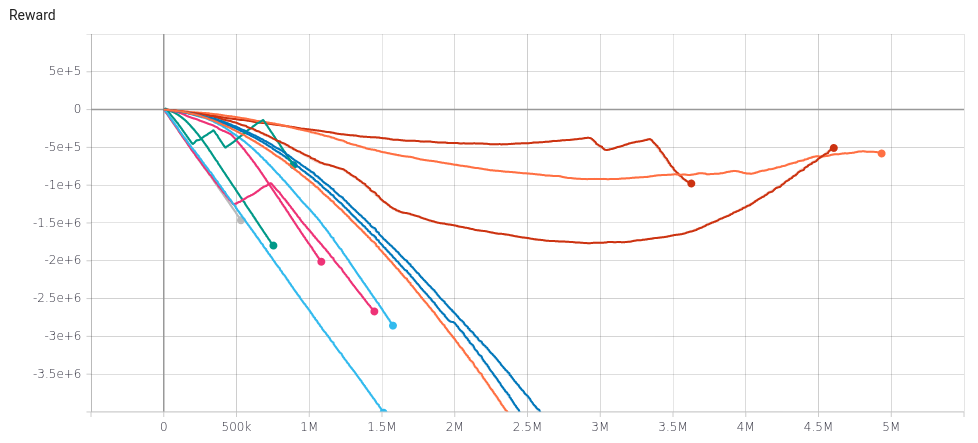
\includegraphics[width=0.8\linewidth,clip=]{images/tensorboard_results.png}%
	\figcaption{Rezultati učenja}%
	\label{fig:tensorboard_results}%
\end{minipage}
\\[\intextsep]

Od svih rezultata bi se moglo odvojiti jedan agent kojemu je vidljivo da mu se nagrada, nakon nekog vremena, stalno boboljšava. Taj jedan agent na kraju treninga, koji se vrtio u periodu od milijun epizoda, posjedije najvišu nagradu. Hiperparametri tog agenta su $10^{-4}$ za stopu učenja, $0.999$ za stopu popusta buduće nagrade te propadanje stope istraživanja $10^{-6}$ u svakoj epizodi do $0.1$ tokom treninga. U igri sa tri agenta koji nasumično donose odluku šansa za pobjedu ja malo priko 30\%, međutim nakon miljun epizoda treninga agent sa neuronskon mrežon je u stanju pobjediti u 40\% slučajeva, što je prikazano slikom~\ref{fig:agent_results}.
\\[\intextsep]
\begin{minipage}{\linewidth}
	\centering%
	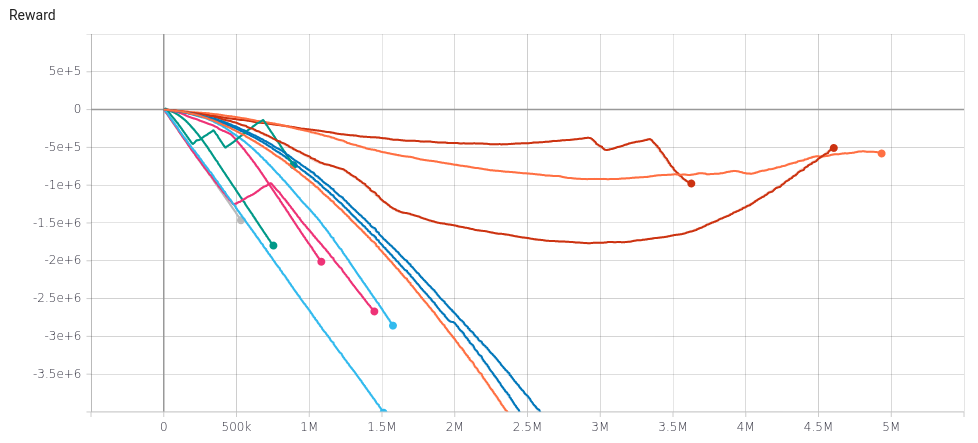
\includegraphics[width=0.8\linewidth,clip=]{images/tensorboard_results.png}%
	\figcaption{Rezultati učenja}%
	\label{fig:agent_results}%
\end{minipage}
\\[\intextsep]